%%%%%%%%%%%%%%%%%%%%%%%%%%%%%%%%%%%%%%%%%
% Beamer Presentation
% LaTeX Template
% Version 1.0 (10/11/12)
%
% This template has been downloaded from:
% http://www.LaTeXTemplates.com
%
% License:
% CC BY-NC-SA 3.0 (http://creativecommons.org/licenses/by-nc-sa/3.0/)
%
%%%%%%%%%%%%%%%%%%%%%%%%%%%%%%%%%%%%%%%%%

%----------------------------------------------------------------------------------------
%	PACKAGES AND THEMES
%----------------------------------------------------------------------------------------

\documentclass{beamer}

\mode<presentation> {

% The Beamer class comes with a number of default slide themes
% which change the colors and layouts of slides. Below this is a list
% of all the themes, uncomment each in turn to see what they look like.

%\usetheme{default}
%\usetheme{AnnArbor}
%\usetheme{Antibes}
%\usetheme{Bergen}
%\usetheme{Berkeley}
%\usetheme{Berlin}
%\usetheme{Boadilla}
%\usetheme{CambridgeUS}
%\usetheme{Copenhagen}
%\usetheme{Darmstadt}
%\usetheme{Dresden}
%\usetheme{Frankfurt}
%\usetheme{Goettingen}
%\usetheme{Hannover}
%\usetheme{Ilmenau}
%\usetheme{JuanLesPins}
%\usetheme{Luebeck}
%\usetheme{Madrid}
\usetheme{Malmoe}
%\usetheme{Marburg}
%\usetheme{Montpellier}
%\usetheme{PaloAlto}
%\usetheme{Pittsburgh}
%\usetheme{Rochester}
%\usetheme{Singapore}
%\usetheme{Szeged}
%\usetheme{Warsaw}

% As well as themes, the Beamer class has a number of color themes
% for any slide theme. Uncomment each of these in turn to see how it
% changes the colors of your current slide theme.

%\usecolortheme{albatross}
%\usecolortheme{beaver}
%\usecolortheme{beetle}
%\usecolortheme{crane}
%\usecolortheme{dolphin}
%\usecolortheme{dove}
%\usecolortheme{fly}
%\usecolortheme{lily}
%\usecolortheme{orchid}
%\usecolortheme{rose}
%\usecolortheme{seagull}
%\usecolortheme{seahorse}
%\usecolortheme{whale}
%\usecolortheme{wolverine}

%\setbeamertemplate{footline} % To remove the footer line in all slides uncomment this line
%\setbeamertemplate{footline}[page number] % To replace the footer line in all slides with a simple slide count uncomment this line

%\setbeamertemplate{navigation symbols}{} % To remove the navigation symbols from the bottom of all slides uncomment this line
}

\usepackage{graphicx} % Allows including images
\usepackage{booktabs} % Allows the use of \toprule, \midrule and \bottomrule in tables
\usepackage{listings}


% -------------------------------------------
% --- Added by me!
\lstMakeShortInline{!}

\usepackage{tikz}
\usetikzlibrary{positioning,calc}
\tikzset{onslide/.code args={<#1>#2}{%
  \only<#1>{\pgfkeysalso{#2}} % \pgfkeysalso doesn't change the path
}}

\makeatletter
\newenvironment<>{btHighlight}[1][]
{\begin{onlyenv}#2\begingroup\tikzset{bt@Highlight@par/.style={#1}}\begin{lrbox}{\@tempboxa}}
{\end{lrbox}\bt@HL@box[bt@Highlight@par]{\@tempboxa}\endgroup\end{onlyenv}}

\newcommand<>\btHL[1][]{%
  \only#2{\begin{btHighlight}[#1]\bgroup\aftergroup\bt@HL@endenv}%
}
\def\bt@HL@endenv{%
  \end{btHighlight}%   
  \egroup
}
\newcommand{\bt@HL@box}[2][]{%
  \tikz[#1]{%
    \pgfpathrectangle{\pgfpoint{1pt}{0pt}}{\pgfpoint{\wd #2}{\ht #2}}%
    \pgfusepath{use as bounding box}%
    \node[anchor=base west, fill=orange!30,outer sep=0pt,inner xsep=1pt, inner ysep=0pt, rounded corners=3pt, minimum height=\ht\strutbox+1pt,#1]{\raisebox{1pt}{\strut}\strut\usebox{#2}};
  }%
}
\makeatother

\usepackage{caption}
\captionsetup{font=scriptsize,labelfont=scriptsize,justification=centering}

% -----------------------------------------------------

%----------------------------------------------------------------------------------------
%	TITLE PAGE
%----------------------------------------------------------------------------------------

\title[Host Compiled Simulation]{Host Compiled Simulation\\for Timing and Power Estimation} % The short title appears at the bottom of every slide, the full title is only on the title page

\author{Gaurav Kukreja \\ Bo Wang} % Your name
\institute[TUM] % Your institution as it will appear on the bottom of every slide, may be shorthand to save space
{
Intel Mobile Communications\\ % Your institution for the title page
}

\date{\today} % Date, can be changed to a custom date

\begin{document}

\definecolor{codegray}{rgb}{0.5,0.5,0.5}
\definecolor{mygreen}{rgb}{0,0.8,0.6}
\definecolor{myorange}{rgb}{1.0,0.4,0}

\lstset{frame=single,
  language=C++,
  aboveskip=3mm,
  belowskip=3mm,
  showstringspaces=false,
  basicstyle={\fontsize{7}{9}\selectfont\ttfamily},
  commentstyle={\itshape\color{codegray}},
  numberstyle={\fontsize{4}{6}\selectfont\ttfamily\color{codegray}},
  keywordstyle=\color{mygreen},
  stringstyle=\color{myorange},
  columns=flexible,
  numbers=left,
  xleftmargin=3em,
  framexleftmargin=2em,
  breaklines=true,
  breakatwhitespace=true,
  tabsize=4,
  captionpos=b,
  moredelim={**[is][\btHL<1>]{@1}{@}},
  moredelim={**[is][\btHL<2>]{@2}{@}}
}

\begin{frame}
\titlepage % Print the title page as the first slide
\end{frame}

\begin{frame}
\frametitle{Overview} % Table of contents slide, comment this block out to remove it
\tableofcontents[
  currentsection,
  sectionstyle=show,
  subsectionstyle=hide
]
\end{frame}

%----------------------------------------------------------------------------------------
%	PRESENTATION SLIDES
%----------------------------------------------------------------------------------------

%------------------------------------------------
\section{Introduction} 
%------------------------------------------------

\subsection{Simulation}
\begin{frame}
\frametitle{Simulation}
Simulation is the technique to imitate the behaviour of a system.
\begin{itemize}
\item Widely used in Hardware Software Co-development.
\item Use cases are performance analysis, functional verification etc.
\end{itemize}
\end{frame}

\begin{frame}
\frametitle{Simulation: Popular Techniques}
\textbf{Cycle Accurate Simulation}
\begin{itemize}
\item Detailed simulation of processor micro-architecture.
\item \textcolor{green}{Cycle Accurate estimation of performance.}
\item \textcolor{red}{Difficult to develop, Very Slow execution.}
\end{itemize}
\textbf{Functional Simulation}
\begin{itemize}
\item High Level of Abstraction.
\item \textcolor{green}{Simple to develop, and fast execution.}
\item \textcolor{red}{Focus is Functional Verification. Cannot be used for performance estimation.}
\end{itemize}
\end{frame}

\subsection{Focus}
\begin{frame}
\frametitle{Our Focus}
A technique for fast simulation of embedded processors that is,
\begin{itemize}
\item Easy to Develop.
\item Fast to Execute.
\item Highly Accurate in Performance Estimation.
\end{itemize}
\end{frame}

\subsection{Related Work}
\begin{frame}
	\frametitle{Related Work}
	\textbf{Sampling Based Approach}
	\begin{itemize}
		\item Small Samples Executed using CAS.
		\item Rest execution fast-forwarded using Functional Simulation.
		\item Results Interpolated.
		\item \textcolor{red}{Inaccurate, Difficult to develop (CAS)}
	\end{itemize}
\end{frame}

\subsection{Host Compiled Simulation}
\begin{frame}
\frametitle{Host Compiled Simulation}
\textbf{Host Compiled Simulation}
\begin{itemize}
\item Based on technique of Source Code Instrumentation.
\item Instrumented code compiled and run on Host Machine, hence the name.
\item Easy to understand, develop and maintain.
\item Fast Execution, and accurate results.
\end{itemize}
\end{frame}

\section{Simple Example}

\begin{frame}[fragile]
\frametitle{Simple Example}
%\textbf{Short Example}
%\begin{columns}
\begin{minipage}{.5\textwidth}
\begin{lstlisting}[title={Simple C Code},label={lst:sumCCode}]
int sum(int array[20])
{
    int i;
    int sum = 0;
	
    for (i=0; i<20; i++)
        sum += array[i];
	
    return sum;
}
\end{lstlisting}
\end{minipage}%
\begin{minipage}{.5\textwidth}
\begin{lstlisting}[title={Objdump Code},label={lst:sumObjCode}]
00008068 <sum>:
8068:     mov     r3, #0
806c:     mov     r2, r3
8070:     ldr     r1, [r0, r3]
8074:     add     r2, r2, r1
8078:     add     r3, r3, #4
807c:     cmp     r3, #80 ; 0x50
8080:     bne     8070 <sum+0x8>
8084:     mov     r0, r2
8088:     bx      lr
\end{lstlisting}
\end{minipage}
\end{frame}

\begin{frame}[fragile]
\frametitle{Simple Example}
%\textbf{Short Example}
%\begin{columns}
\begin{minipage}{.5\textwidth}
\begin{lstlisting}[title={Simple C Code},label={lst:sumCCode}]
int sum(int array[20])
{
    int i;
    int sum = 0;
	
    for (i=0; i<20; i++)
        sum += array[i];
	
    return sum;
}
\end{lstlisting}
\end{minipage}%
\begin{minipage}{.5\textwidth}
\begin{lstlisting}[title={Objdump Code},label={lst:sumObjCode}]
00008068 <sum>:
8068:     mov     r3, #0
806c:     mov     r2, r3
8070:     ldr     r1, [r0, r3]
8074:     add     r2, r2, r1
8078:     add     r3, r3, #4
807c:     cmp     r3, #80 ; 0x50
8080:     bne     8070 <sum+0x8>
8084:     mov     r0, r2
8088:     bx      lr
\end{lstlisting}
\end{minipage}
\vspace*{-15pt}
\begin{table}[b]
\fontsize{8}{10}\selectfont
\begin{center}
\begin{tabular}{cccc}
\toprule
	\multicolumn{2}{c}{Basic Block in Binary} & \multicolumn{2}{c}{Matching block in Source}\\ 
	\midrule
	BlockID & Lines & BlockID & Lines \\
    \hline
	1 & 2-3 & 1 & 3-4 \\
	2 & 4-8 & 2 & 7 \\
	3 & 9-10 & 3 & 9 \\	
\bottomrule
\end{tabular}
%\caption{Mapping of Basic Blocks}
\end{center}
\end{table}
\end{frame}

\begin{frame}[fragile]
\frametitle{Instrumented Code}
\begin{minipage}{.62\textwidth}
\begin{lstlisting}[label={lst:sumInstCode},
                    basicstyle={\fontsize{6}{8}\selectfont\ttfamily}]
@1unsigned int execCycles;@
@1unsigned int memAccessCycles;@

int sum(int array[20])
{
    int i;
    int sum = 0;
    @1execCycles += 2;@
    @1memAccessCycles += simICache(0x8068, 8);@
	
    for (i=0; i<20; i++)
    {
        sum += array[i];
        @1memAccessCycles += simDCache(array + i, READ);@
        @1execCycles += 5;@
        @1memAccessCycles += simICache(0x8070, 40);@
    }
	
    @1execCycles += 2;@
    @1memAccessCycles += simICache(0x8084, 8);@
    return sum;
}
\end{lstlisting}
\end{minipage}%
\begin{minipage}{0.38\textwidth}
\begin{lstlisting}[basicstyle={\fontsize{6}{8}\selectfont\ttfamily},aboveskip=1.5mm,belowskip=0mm]
int sum(int array[20])
{
    int i;
    int sum = 0;
	
    for (i=0; i<20; i++)
        sum += array[i];
	
    return sum;
}
\end{lstlisting}
\begin{lstlisting}[basicstyle={\fontsize{6}{8}\selectfont\ttfamily},aboveskip=4.25mm,belowskip=0mm]
00008068 <sum>:
8068:     mov     r3, #0
806c:     mov     r2, r3
8070:     ldr     r1, [r0, r3]
8074:     add     r2, r2, r1
8078:     add     r3, r3, #4
807c:     cmp     r3, #80 ; 0x50
8080:     bne     8070 <sum+0x8>
8084:     mov     r0, r2
8088:     bx      lr
\end{lstlisting}
\end{minipage}
\end{frame}

%\begin{frame}
%\frametitle{Contribution}
%\begin{itemize}
%\item Algorithm for Mapping between Source and Binary Code.
%\item Detailed Cache Simulation for better accuracy.
%\item Accurate Simulation of Processor Pipeline.
%\item Using Power State Model for Power Estimation.
%\end{itemize}
%\end{frame}

\begin{frame}
\frametitle{Objective}
\begin{itemize}
\item Develop a tool for Automatic Instrumentation.
\item ARM Cortex A5 based processor as reference target device.
\item Bare-Metal Applications.
\item Generate Time and Power Consumption Estimates.
\end{itemize}
\end{frame}

%------------------------------------------------

\section{Timing Estimation}

%\subsection{Outline}
%
%\begin{frame}
%\frametitle{Outline of our Approach}
%\begin{itemize}
%\item Generate Mapping between Source Code and Binary Code.
%\item Extract Information from GDB
%\item Data Cache Simulation
%\item Instruction Cache Simulation
%\item Annotation for cycles spent in Pipeline
%\end{itemize}
%\end{frame}

\subsection{Mapping between Source and Binary}

\begin{frame}
\frametitle{Mapping between Source and Binary}
\begin{itemize}
\item Very important for accurate instrumentation.
\item Compiler destroys mapping during optimization phases.
\item GDB provides mapping, but highly inaccurate.
\item Control Flow Analysis to generate mapping between Basic Blocks.
\end{itemize}
\end{frame}

\begin{frame}
\frametitle{Mapping between Source and Binary}
In this project, mapping is generated using following steps.
\begin{itemize}
\item Cross-Compile Source Code.
\item Convert IR Code to C Code (Intermediate Source Code).
\item Extract CFG from ISC and Binary Code.
\item Map CFGs using Mapping Algorithm
\end{itemize}
\end{frame}

\begin{frame}
\frametitle{Conversion of IR Code to C Code}
\begin{figure}
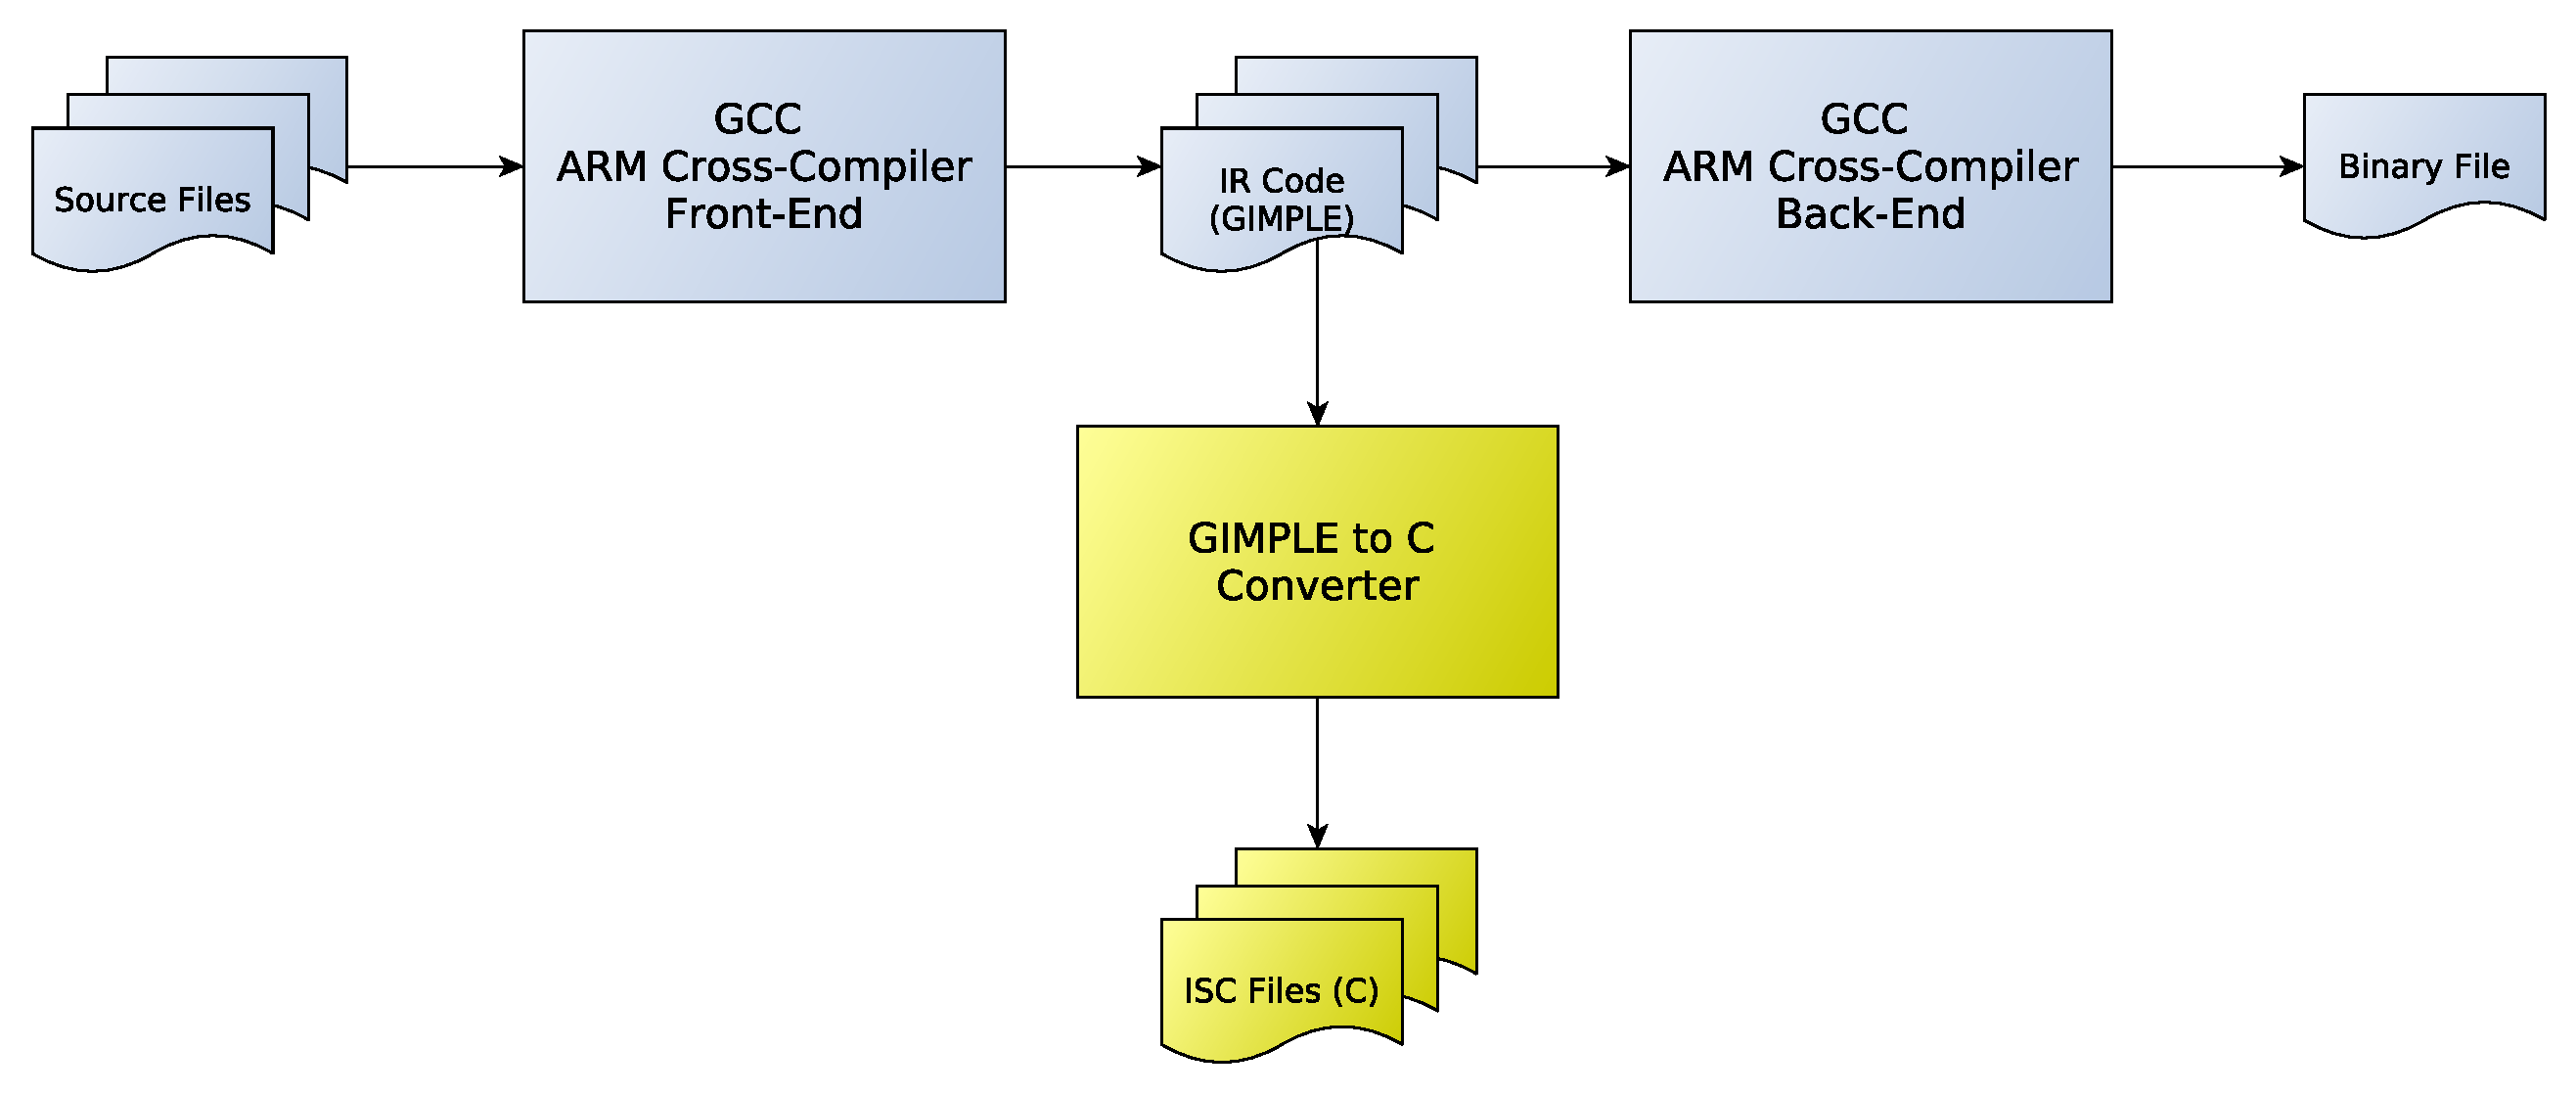
\includegraphics[width=\textwidth]{figures/ir2cConversion.pdf}
\end{figure}
\tiny{* Code for GIMPLE to C converter reused from RBA project [TODO]}
\end{frame}

\begin{frame}
\frametitle{Mapping Algorithm}
\begin{itemize}
\item Extract CFG from ISC and Binary Code.
\item Graph Matching Algorithm using Depth First Traversal.
\item Special handling for each optimization.
\item GDB Debug information in Corner Cases.
\end{itemize}
\end{frame}

\begin{frame}[fragile]
\frametitle{Handling of Compiler Optimization : Conditional Execution}
\begin{minipage}{.5\textwidth}
\begin{lstlisting}[title={Simple C Code},label={lst:sumCCode}]
...
if (a > b)
    max = a;
else
    max = b;
...
\end{lstlisting}
\begin{figure}
\vspace*{-20pt}
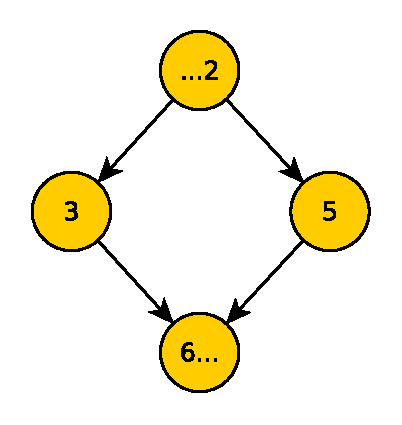
\includegraphics[width=80pt]{figures/CondExecSrcFlowChart.pdf}
\end{figure}
\end{minipage}%
\begin{minipage}{.5\textwidth}
\begin{lstlisting}[title={Unoptimized Assembly Code},label={lst:sumObjCode}]
806c:     ...
8070:     cmp     r1, r2
8074:     ble     8080
8078:     mov     r3, r1
807c:     b       8084
8080:     mov     r3, r2
8084:     ...
\end{lstlisting}
\begin{figure}
\vspace*{-20pt}
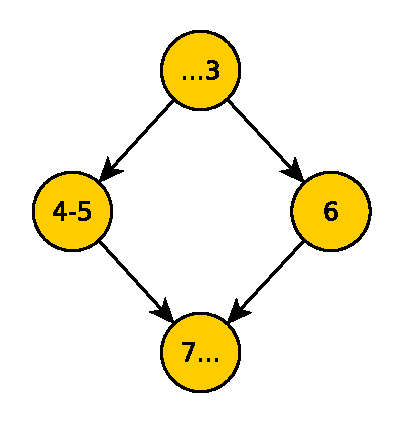
\includegraphics[width=80pt]{figures/CondExecObjUnoptFlowChart.pdf}
\end{figure}
\end{minipage}
\end{frame}

\begin{frame}[fragile]
\frametitle{Handling of Compiler Optimization : Conditional Execution}
\begin{minipage}{.5\textwidth}
\begin{lstlisting}[title={Simple C Code},label={lst:sumCCode}]
...
if (a > b)
    max = a;
else
    max = b;
...
\end{lstlisting}
\begin{figure}
\vspace*{-20pt}
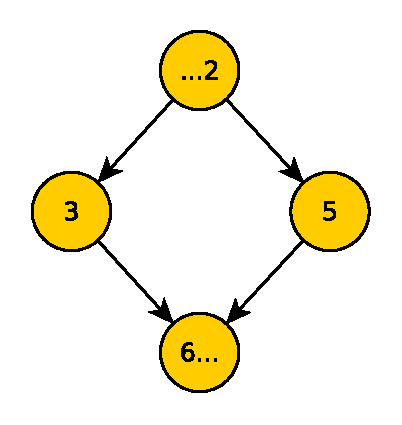
\includegraphics[width=80pt]{figures/CondExecSrcFlowChart.pdf}
\end{figure}
\end{minipage}%
\begin{minipage}{.5\textwidth}
\begin{lstlisting}[title={Optimized Assembly Code},label={lst:sumObjCode}]
806c:     ...
8070:     cmp     r1, r2
8074:     movgt   r3, r1
8078:     movle   r3, r2
807c:     ...
\end{lstlisting}
\begin{figure}
\vspace*{20pt}
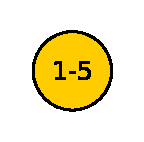
\includegraphics[width=40pt]{figures/CondExecObjOptFlowChart.pdf}
\end{figure}
\end{minipage}
\end{frame}

\begin{frame}
%TODO: Fix the image!!
\begin{minipage}{.5\textwidth}
\begin{figure}
\includegraphics[width=.5\textwidth]{figures/obj_my_ctop_IR_adpcm_coder-crop}
\end{figure}
\end{minipage}%
\begin{minipage}{.5\textwidth}
\begin{figure}
\includegraphics[height=.9\textheight]{figures/isc_adpcm_IR_adpcm_coder-crop}
\end{figure}
\end{minipage}
\end{frame}

\subsection{Annotation for Cycles spent in Pipeline}

\begin{frame}
\frametitle{Annotation for Cycles spent in Pipeline}
Performed at Basic Block Granularity.\\
\vspace*{20pt}
Important to consider
\begin{itemize}
\item Pipeline Architecture of the target processor.
\item Data and Control Hazards, that leads to pipeline stalls.
\item Branch Prediction, that prevents pipeline flushes.
\end{itemize}
\end{frame}

\begin{frame}
\frametitle{Pipeline architecture of ARM Cortex A5}
The ARM Cortex A5 has an 8-stage pipeline.
\begin{figure}
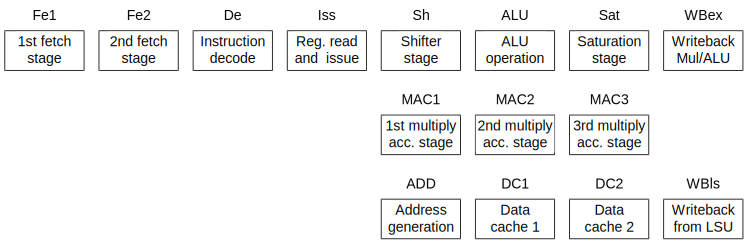
\includegraphics[width=\textwidth]{figures/pipeline}
\end{figure}
Lets assume,
\begin{itemize}
\item Pipeline is empty at start of Basic Block.
\item All data is available without latency.
\end{itemize}
\end{frame}

%\begin{frame}
%\frametitle{Effects due to Data and Control Hazards}
%Instructions are executed in a sequence in the processor pipeline. An instruction may need to use data produced by the previous instruction. The result may not be available yet, and the pipeline may need to stall to wait for the data. This situation is called \textbf{Data Hazard}.
%
%Execution Units are used in a processor, which perform instructions like addition, multiplication. Some instructions may need more than one cycle to complete. During this time, the execution unit is reserved. A subsequent instruction may have to wait to use the same execution unit. This is known as \textbf{Control Hazard}.
%
%Compilers try to optimize code by eliminating Data and Control Hazards, but not all can be eliminated.
%\end{frame}

\begin{frame}[fragile]
\frametitle{Effects due to Data and Control Hazards}
For each Basic Block from Binary Code,
\begin{itemize}
\item Parse instructions sequentially.
\item Simulate progress in pipeline.
\item Identify interlocking (hazards) and add penalty.
\item Annotate to mapped block in Source Code.
\end{itemize}
\begin{lstlisting}[numbers=none]
...
for(i<0; i<10; i++) {}
    @1execCycles += 23;@
    sum += array[i];
    ...
}
...
\end{lstlisting}
\end{frame}

\begin{frame}
\frametitle{Branch Prediction}
\begin{itemize}
\item Reduces number of pipeline flushes.
\item Major impact on performance.
\item Branch Prediction Unit is simulated to account for this.
\end{itemize}
\end{frame}

\begin{frame}
\frametitle{Branch Prediction Algorithm}
\begin{itemize}
\item Simulates the BPU on ARM Cortex A5
\item 125 entry Branch History Table.
\item State Machine for each Entry. 2 bit state information.
\end{itemize}
\begin{figure}
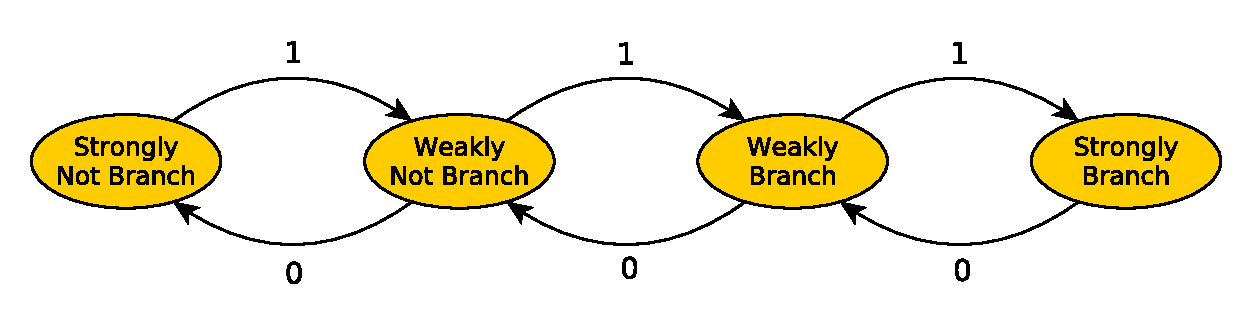
\includegraphics[width=300pt]{figures/BranchPredictionSMD.pdf}
\end{figure}
\end{frame}

\begin{frame}[fragile]
\frametitle{Branch Prediction API}
Branch Prediction Simulator offers following API.
\begin{lstlisting}[frame=none,numbers=none]
/**
 * @brief Function called at the beginning of a Basic Block
 *        to simulate Branch Prediction Unit.
 * 
 * @param Start Address of Basic Block being entered.
 * @param End Address of Basic Block being entered.
 * 
 * @return True, if branch was correctly predicted.
 *           False, if branch was not correctly predicted.
 */
unsigned int branchPred_enter{unsigned long startAdd,
                                 unsigned long endAdd};
\end{lstlisting}
\end{frame}

\begin{frame}[fragile]
\frametitle{Annotation for Branch Prediction}
\begin{itemize}
\item Start and End address of Basic Block extracted from Binary.
\item Annotation done at beginning of Basic Block.
\item Depending on outcome, penalty is subtracted from \texttt{execCycles}.
\end{itemize}
\begin{lstlisting}[numbers=none]
...
for(i=0; i<10; i++) {
    @1execCyles += 23;@
    @1execCycles -= (branchPred_enter(0x348, 0x380) ? 7 : 0);@
    sum += array[i];
    ...
}
...
\end{lstlisting}
\end{frame}

\subsection{Cache Simulation}

\begin{frame}
\frametitle{Cache Simulator}
Cache Hierarchy on target device.
\begin{table}
\centering
\begin{tabular}{c|ccc}
        &  Size   & N-way   & Cache Line Size \\
    \hline
    L1 D Cache  & 32 KB & 4 & 32 B \\
    L1 I Cache  & 32 KB & 2 & 32 B \\
    L2 Cache    & 256 KB & 16 & 32 B \\
\end{tabular}
\end{table}
\begin{itemize}
\item Pseudo Random Replacement Policy
\item Data Prefetching
\end{itemize}
\end{frame}

\begin{frame}[fragile]
\frametitle{Instruction Cache Simulation}
\begin{lstlisting}[frame=none,numbers=none,basicstyle={\fontsize{9}{11}\selectfont\ttfamily}]
/**
 * @brief Function to simulate Instruction Cache Access.
 *
 * @param Start Address of the basic block.
 * @param Size of the basic block in Bytes.
 *
 * @return Number of cycles spent in performing access.
 */
unsigned long long simICache(unsigned long address,
                                unsigned long size);
\end{lstlisting}
\end{frame}

\subsection{Instruction Cache Simulation}

\begin{frame}[fragile]
\frametitle{Instruction Cache Simulation}
\begin{itemize}
\item Start address and size of Basic Blocks extracted from Binary.
\item Annotation at beginning of mapped Basic Block in Source Code.
\item Return value added to \texttt{memAccessCycles}.
\end{itemize}
\begin{lstlisting}
...
for(i=0; i<10; i++) {
    @1execCyles += 23;@
    @1execCycles -= (branchPred_enter(0x348, 0x380) ? 7 : 0);@
    @1memAccessCycles += simICache(0x348, 56);@
    sum += array[i];
    ...
}
...
\end{lstlisting}
\end{frame}

\subsection{Data Cache Simulation}

\begin{frame}[fragile]
\frametitle{Data Cache Simulation}
\begin{lstlisting}[frame=none,numbers=none,basicstyle={\fontsize{9}{11}\selectfont\ttfamily}]
/**
 * @brief Function to simulate Data Cache Access.
 *
 * @param Address of the memory being accessed.
 * @param True, if access is Read Access. 
 *         False, if write access.
 *
 * @return Number of cycles spent in performing access.
 */
unsigned long long simDCache(unsigned long address,
                                unsigned int isReadAccess);
\end{lstlisting}
\end{frame}

\begin{frame}
\frametitle{Data Cache Simulation}
\textcolor{red}{Address from host cannot be used for simulation.}\\
\vspace*{20pt}
Will lead to inaccuracies, because
\begin{itemize}
\item Different sizes of Basic Data Types.
\item Different Memory Alignment on Host and Target.
\end{itemize}
\vspace*{20pt}
Memory Access Reconstruction
\begin{itemize}
\item Inspired by [TODO]
\item Resolve address of each load/store instruction on target device.
\end{itemize}
\end{frame}

\begin{frame}
\frametitle{Memory Access Reconstruction}
\begin{itemize}
\item Resolve Physical Address of each variable in target memory.
\item Identify variable being accessed by each load/store.
\item Identify index information from source code.
\item Simulate Data Cache.
\end{itemize}
\end{frame}

\begin{frame}[fragile]
\frametitle{Resolve Physical Address of Variables}
Global Variables
\begin{itemize}
\item Bare-Metal Execution. Address fixed at compile time.
\item Extracted by Static Analysis of binary.
\end{itemize}
Annotate address in code as follows,
\begin{lstlisting}
unsigned int globVar[100];
@1unsigned long globVar_addr = 0x7c8;@
\end{lstlisting}
\end{frame}

\begin{frame}[fragile]
\frametitle{Resolve Physical Address of Variables}
Local Variable
\begin{itemize}
\item Stored in Stack, address only known at run-time.
\item Address relative to stack, can be known statically.
\item Simulate growth of stack at run-time to resolve physical address.
\end{itemize}
\begin{lstlisting}
@1unsigned long CSIM_SP = 0x1d4c8;@              // Initial Value of SP.

int foo()
{
    @1CSIM_SP += 88;@                            // Size of Stack Frame for foo.

    int localVar;
    @1unsigned long localVar_addr = 0x8;@        // Address relative to SP.
    ...
}
\end{lstlisting}
\end{frame}

\begin{frame}
\frametitle{Identify Load/Store Operations in Binary Code}
To identify variable accessed by a load/store instruction,
\begin{itemize}
\item Binary code is functionally simulated.
\item Register state is maintained, and updated as per instruction.
\item Branch instructions are ignored.
\item Address for each load/store is extracted.
\item Variable being accessed is known.
\end{itemize}
\begin{figure}
\includegraphics[width=150pt]{figures/FuncSimulator-crop.pdf}
\end{figure}
\end{frame}

\begin{frame}[fragile]
\frametitle{Annotation of Memory Access}
To find the line in source code, which causes the memory access operation,
\begin{itemize}
\item Each line is parsed using a custom C Parser.
\item Index information is extracted.
\item Annotation as follows.
\end{itemize}
\begin{lstlisting}
...
for (i=0; i < 100; i++) {
    sum += globalVar[i];
    @1memAccessCycles += simDCache ( globalVar_addr + i * 4, True );@
}
localVar = sum / 100;
@1memAccessCycles += simDCache ( SP + localVar_addr, False );@
...
\end{lstlisting}
\end{frame}

\begin{frame}
\frametitle{Timing Estimation}
\begin{itemize}
\item Annotated Source Code is compiled and run on Host Machine.
\item Time spent in Active state and Idle State of CPU is reported.
\item Additionally, trace information from Cache is generated.
\end{itemize}
\end{frame}

\section{Power Estimation}
\begin{frame}
For estimating power, the power state model approach has been used.
\begin{itemize}
\item Power consumed by each component in active and idle state is known.
\item Trace information for each basic block, shows components that were active and the duration.
\item Total power being consumed at a time, can be estimated.
\end{itemize}
\end{frame}

\begin{frame}
\frametitle{Components for Power Estimation}
\begin{minipage}{.3\textwidth}
\begin{figure}
\includegraphics[width=.8\textwidth]{figures/Components-crop.pdf}
\end{figure}
\end{minipage}%
\begin{minipage}{.7\textwidth}
Target System is divided into components as follows
\begin{itemize}
\item Core and L1 Caches
\item L2 Cache
\item External Memory along with controller and NOC.
\end{itemize}
\end{minipage}
\end{frame}

\section{Conclusion}

\subsection{Test Setup}
\begin{frame}
\frametitle{Test Setup}
For testing, ARM Cortex A5 core was used. Results from ARM Performance Measurement Unit were compared.
\begin{itemize}
\item Number of Cache Misses.
\item Total Cycles.
\end{itemize}
Accurate Prediction of Cache Misses, will verify the correctness of the instrumentation.
\end{frame}

\subsection{Results}
\begin{frame}
\frametitle{ADPCM Benchmark}
\begin{table}[b]
\fontsize{7}{9}\selectfont
\centering
\begin{tabular}{|c|c|c|c|}
\hline
    & HCS & Actual & Accuracy \\
\hline
Total Cache Miss & 91452 & 91604 & 99.99\% \\
Total Cycles & 46110394 & 45594862 & 99.98\% \\
\hline
\end{tabular}
\end{table}
\begin{figure}
\vspace*{-20pt}
\includegraphics[width=200pt]{figures/adpcm_power_10000.png}
\end{figure}
\end{frame}

\begin{frame}
\frametitle{Sieve Benchmark}
\begin{table}[b]
\fontsize{7}{9}\selectfont
\centering
\begin{tabular}{|c|c|c|c|}
\hline
    & HCS & Actual & Accuracy \\
\hline
Total Cache Miss & 933109 & 934250 & 99.88\% \\
Total Cycles & 99068687 & 100403731 & 98.67\% \\
\hline
\end{tabular}
\end{table}
\begin{figure}
\vspace*{-20pt}
\includegraphics[width=200pt]{figures/sieve_power_100000.png}
\end{figure}
\end{frame}

\end{document} 